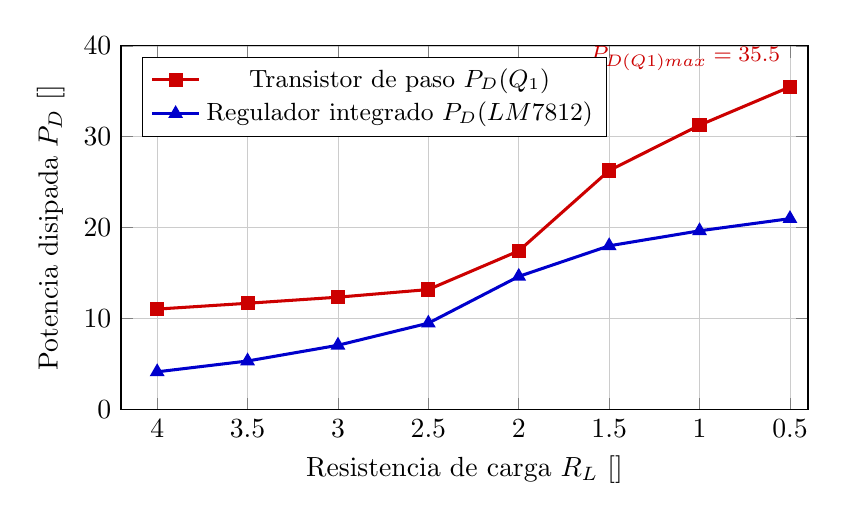
\begin{tikzpicture}
\begin{axis}[
    width=0.85\textwidth,
    height=6.2cm,
    xlabel={Resistencia de carga $R_L$ [\si{\ohm}]},
    ylabel={Potencia disipada $P_D$ [\si{\watt}]},
    grid=both,
    grid style={line width=.1pt, draw=gray!20},
    major grid style={line width=.2pt, draw=gray!40},
    x dir=reverse,
    xmin=0.4, xmax=4.2,
    ymin=0, ymax=40,
    legend pos=north west,
    legend style={font=\small}
]

% Potencia Q1
\addplot[
    color=red!80!black,
    mark=square*,
    mark size=2pt,
    line width=1.1pt
] coordinates {
    (4.0, 11.04)
    (3.5, 11.68)
    (3.0, 12.35)
    (2.5, 13.19)
    (2.0, 17.44)
    (1.5, 26.28)
    (1.0, 31.27)
    (0.5, 35.48)
};
\addlegendentry{Transistor de paso $P_D(Q_1)$}

% Potencia LM7812
\addplot[
    color=blue!80!black,
    mark=triangle*,
    mark size=2pt,
    line width=1.1pt
] coordinates {
    (4.0, 4.14)
    (3.5, 5.33)
    (3.0, 7.06)
    (2.5, 9.49)
    (2.0, 14.63)
    (1.5, 18.00)
    (1.0, 19.65)
    (0.5, 20.99)
};
\addlegendentry{Regulador integrado $P_D(\text{LM7812})$}

% Limite disipador TO-220
\node[anchor=south east, text=red!80!black, font=\footnotesize] at (axis cs: 0.5, 36.2) {$P_{D(Q1)max} = \SI{35.5}{\watt}$};

\end{axis}
\end{tikzpicture}
